
\chapter{Application}
\label{cha:application}

This chapter present two more involved cases of identification. The first case
is identification of the COST beam, introduced as a standard test case for
polynomial nonlinearities, ie. two polynomial nonlinearities at the same DOF.
The second case demonstrate the usage of cubic spines to identify a system with
two different clearances. The clearance distances are also found.


\section{COST beam}
\label{sec:cost-beam}

The European action COST F3 nonlinear beam \autocite{GOLINVAL2003} was
introduced in 2003 as a benchmark system for nonlinear vibrations. The
experimental setup is shown in fig. \ref{fig:beam_setup} and consists of a
clamped beam with a thin beam part at the end of the main beam.

\begin{figure}[!ht]
  \centering
  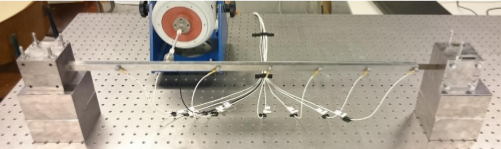
\includegraphics[width=0.7\textwidth]{nlbeam/beam_setup.png}
  \caption{Experimental setup for the COST beam. The setup is vertical to avoid
    gravitational effects which cannot be ignored due to the thin beam.}
  \label{fig:beam_setup}
\end{figure}

Accelerations are measured evenly along the beam at seven locations and excited
at node two.
From \textcite{lenaerts2003a} is it known that the system exhibit a (geometric)
cubic nonlinearity due to large deformations of the thin beam and quadratic
nonlinearity due to the clamped connection, both located at the tip of the main
beam. Using data given at the Nolinsys course, the beam will be identified as an
example of a MIMO system. After successful identification a FE model is built
using the identified parameters, and used for further examination.


\subsection{Identification}

The time series were obtained by Nolinsys. The beam is excited with a periodic
broadband input with flat amplitude spectrum, i.e. a multisine at low and high
level. At low and high level, the beam behaves linear and nonlinear
respectively. To avoid leakage in the identification due to transient behavior,
the periods used are selected from a plot of the periodicity. From fig.
\ref{fig:nlbeam_per} is seen that transients are apparent in the first two
periods and not apparent in periods 4-7, which are used for the identification.

\begin{figure}[!ht]
  \centering
  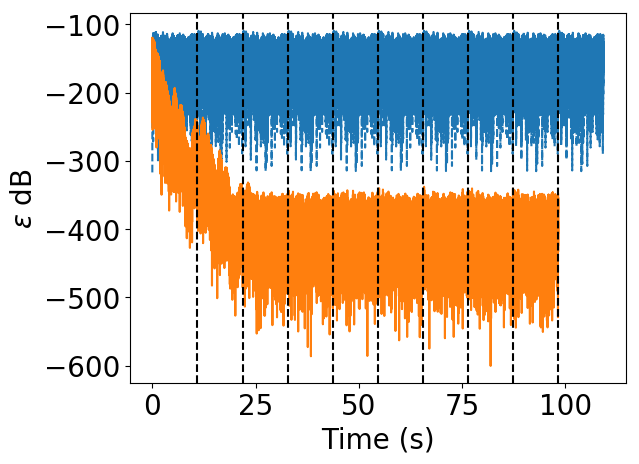
\includegraphics[width=0.6\textwidth]{nlbeam/fnsi/per.png}
  \caption{Periodicity of recorded signal at high level wrt. the last period.
    Measured at the nonlinear dof.}
  \label{fig:nlbeam_per}
\end{figure}

Figure \ref{fig:nlbeam_stab} shows the stabilisation diagram used for determine
model order. Fig. \ref{fig:nlbeam_stab}(a) is used for linear identification and
is fully stabilised at order 6. Fig. \ref{fig:nlbeam_stab}(b) shows the
nonlinear system identified with linear analysis, ie. without specifying
nonlinear basis functions. The first mode does not stabilise, which normally
indicates that the supplied basis functions are inadequate to represent the
nonlinearity. Fig. \ref{fig:nlbeam_stab}(c) shows the stabilisation after
supplying a quadratic and cubic basis function. The first mode stabilises at
model order 6, ie. the identification is most likely trustworthy and the
nonlinearity are described by these functions.

\begin{figure}
  \centering
    \begin{subfigure}[b]{0.45\textwidth}
      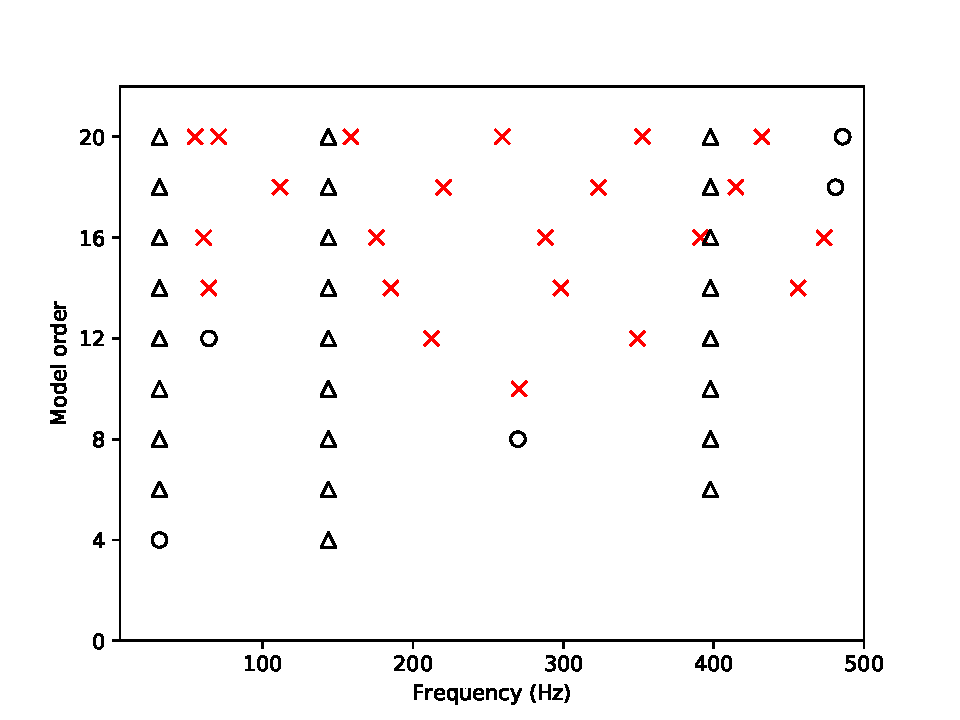
\includegraphics[width=\linewidth]{nlbeam/fnsi/stab_lin.pdf}
    \end{subfigure}
    ~
    \begin{subfigure}[b]{0.45\textwidth}
      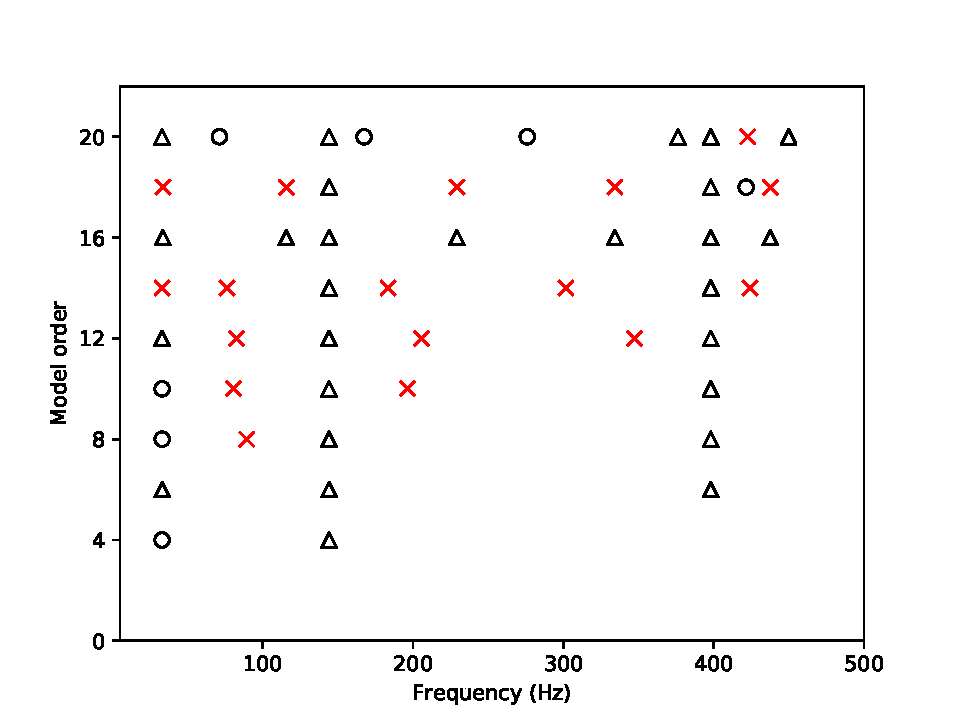
\includegraphics[width=\linewidth]{nlbeam/fnsi/stab_nlin1.pdf}
    \end{subfigure}
    \\
    \begin{subfigure}[b]{0.45\textwidth}
      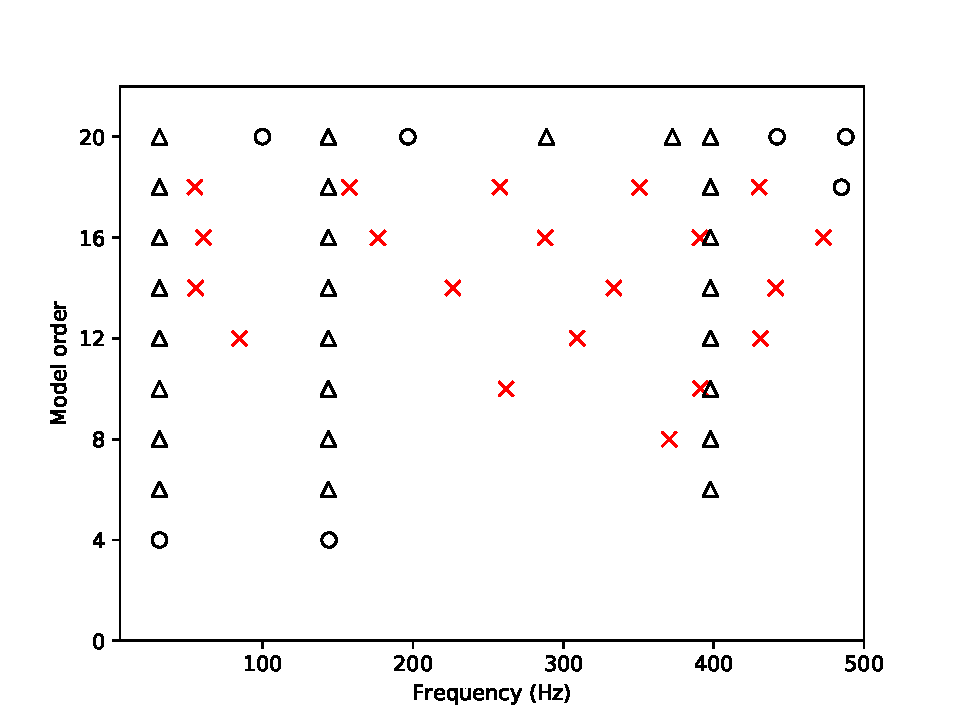
\includegraphics[width=\linewidth]{nlbeam/fnsi/stab_nlin2.pdf}
    \end{subfigure}
    \caption{Estimation of model order.
    $\pmb\times$(red): new pole;
    $\pmb\star$: stabilisation in natural frequency;
    $\pmb\square$: extra stabilisation in damping ratio;
    $\pmb\circ$: extra stabilisation in MACX;
    $\pmb\triangle$: full stabilisation.
    Stabilisation thresholds in natural frequency, damping ratio and MACX value
    are $0.5\%, 2\%, 0.98$, respectively. Not all types of stabilisation are
    present here.
    \textbf{(a)}: Low level, linear identification;
    \textbf{(b)}: High level, linear identification - no stabilisation of first mode;
    \textbf{(c)}: High level, nonlinear identification - stabilisation of first mode;
  }
  \label{fig:nlbeam_stab}
\end{figure}

The identified linear parameters are shown in table \ref{nlbeam_par}. As
expected, the first mode shows a hardening which is seen by the linear
identification at high level. The linear parameters are estimated correctly at
high level using the two basis functions.

\begin{center}
  \begin{tabular}{*{4}{c}}
    \hline
    Mode & Frequency (Hz) & Damping ration (\%) & Deviation from linear freq. (\%) \\
    \hline
    1 & 31.3 & 1.27 \\
    2 & 143.6 & 0.29 \\
    3 & 397.8 & 0.14 \\
    \hline
    1 & 33.1 & 1.08 & 5.7 \\
    2 & 144.1 & 0.29 & 0.3 \\
    3 & 398.0 & 0.14 & 0.05 \\
    \hline
    1 & 31.3 & 1.27 & $10^{-3}$ \\
    2 & 143.6 & 0.29 & $10^{-5}$ \\
    3 & 397.8 & 0.14 & $10^{-6}$ \\
    \hline
  \end{tabular}
  \captionof{table}{Estimated linear natural frequencies and damping ratios for
    the COST beam.
    \textbf{(upper)}: Low level, linear identification;
    \textbf{(middle)}: High level, linear identification;
    \textbf{(lower)}: High level, nonlinear identification.
  }
  \label{tab:nlbeam_par}
\end{center}

The identified nonlinear coefficients are shown in figure \ref{fig:nlbeam_knl}.
The deviation of the real part is just within 1\% and the imaginary part are
around three orders of magnitude smaller, indicating a good identification.

\begin{figure}[!ht]
  \centering
  \begin{subfigure}[b]{0.45\textwidth}
    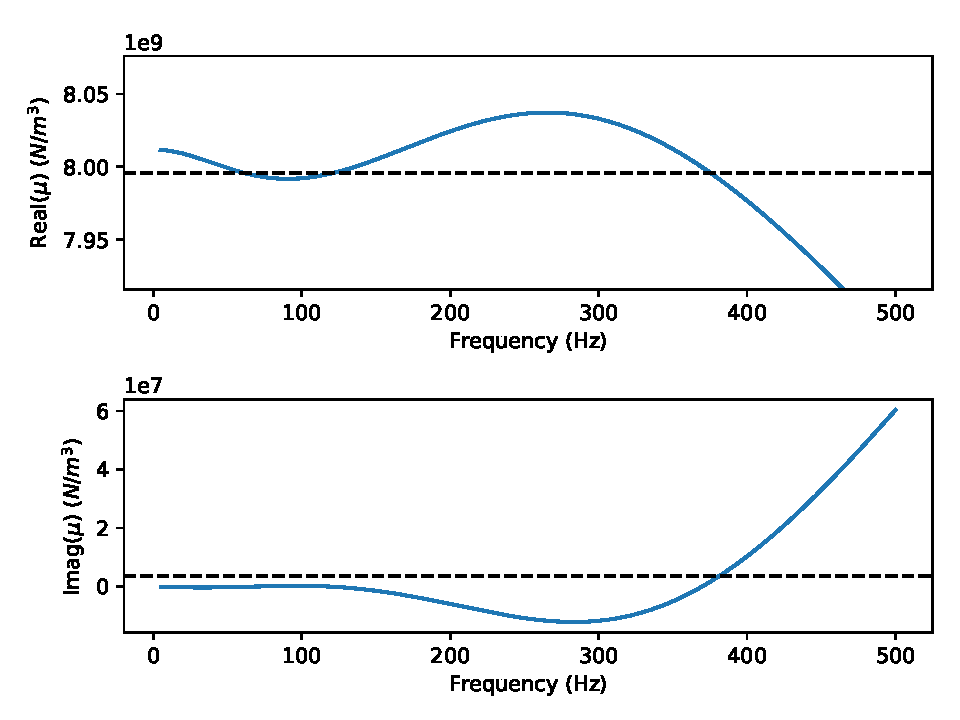
\includegraphics[width=\linewidth]{nlbeam/fnsi/knl0.pdf}
    \caption{}
  \end{subfigure}
  ~
  \begin{subfigure}[b]{0.45\textwidth}
    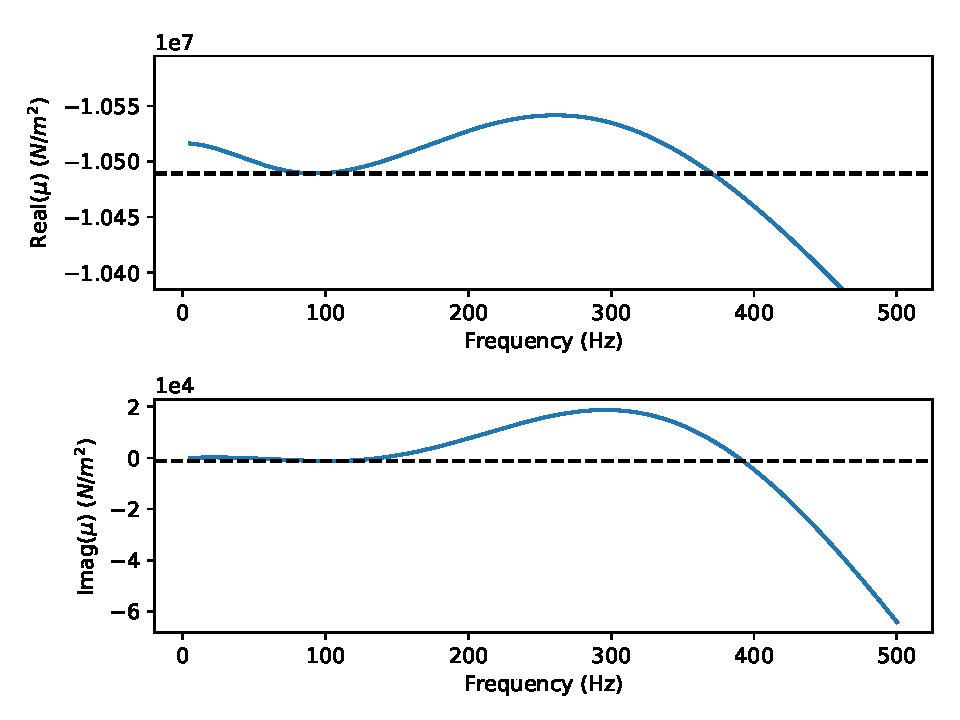
\includegraphics[width=\linewidth]{nlbeam/fnsi/knl1.pdf}
    \caption{}
  \end{subfigure}
  \caption{Real and imaginary part of estimated nonlinear coefficients $\mu_1$
    and $\mu_2$. The variation of Re($\mu$) is seen to be within a 1 interval.
    The imaginary part is about three orders of magnitude smaller. Both
    indicates a good quality of the estimation. The spectral averages of the
    real part and ratio $\text{log}_{10}\frac{\Re(\mu)}{\Im(\mu)}$ are:
    \textbf{(a)}: $\mu_1 = 8.0 \times 10^9 m/n^3$, ratio = 3.34;
    \textbf{(b)}: $\mu_2 = -1.05 \times 10^7 m/n^2$, ratio = 3.96.
  }
  \label{fig:nlbeam_knl}
\end{figure}


Finally fig. \ref{fig:nlbeam_frf} shows the FRF. Nonlinear distortion is seen
from the signal at high level excitation. The FRF(blue) from low level excitation and
identified by FNSI with basis functions(green) match.

\begin{figure}[!ht]
  \centering
  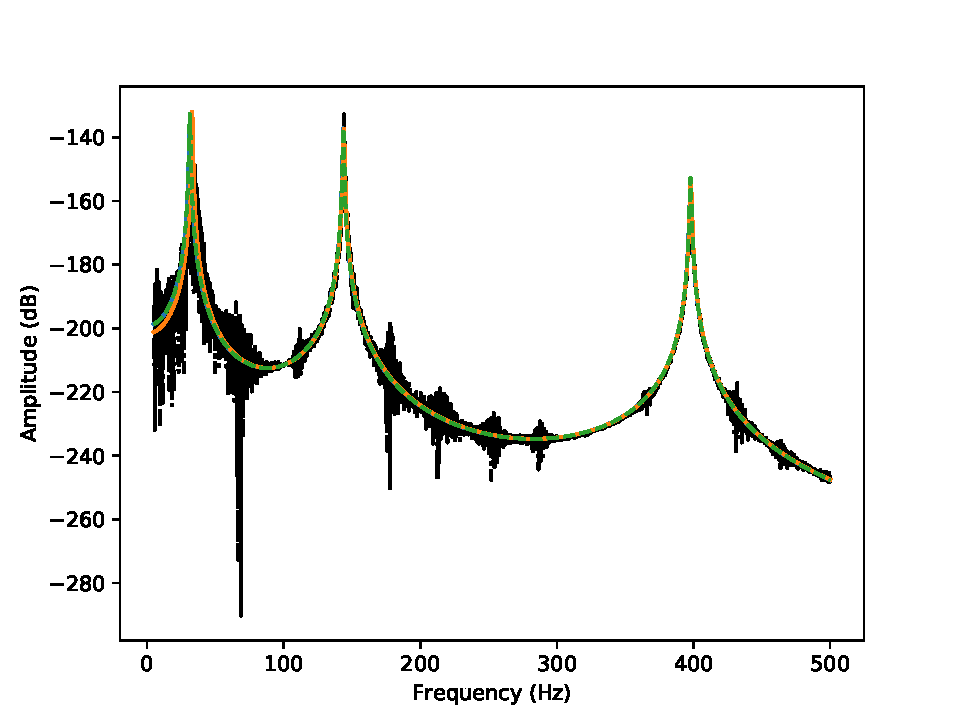
\includegraphics[width=0.6\textwidth]{nlbeam/fnsi/frf.pdf}
  \caption{FRF. Nonparametric(NP) is FRF directly from signal, parametric is
    identified FRF.
    \sampleline{}: NP from high level excitation;
    \textcolor{blue}{\sampleline{}}: NP from low level excitation.
    \textcolor{orange}{\sampleline{}}: Linear parametric from high level excitation.
    \textcolor{green}{\sampleline{dashed}}: nonlinear parametric from high level excitation.
}
  \label{fig:nlbeam_frf}
\end{figure}

\subsection{Design}

The test setup is modelled as shown in fig \ref{fig:nlbeam_fem}, using 14 and 3
two-dimensional Bernoulli-Euler beam elements for the main and thin beam
respectively. The connection between the two beams is modelled by an additional
linear rotational stiffness, as suggested in \autocite{lenaerts2003a}, resulting
in a model with 35 dofs.
% In traditional FEM, boundary conditions can be enforced
% in different ways; either modifying the stiffness matrix or the load vector.
% With the methods presented here, boundary conditions should always be enforced
% by modifying the stiffness matrix, i.e. for fixed dofs all rows and columns
% relating to these dofs are removed, which is why the system ends up having 35
% dofs.

\begin{figure}[!ht]
  \centering
  \def\svgwidth{6cm}
  \import{fig/nlbeam/}{beam_fem.pdf_tex}
  \caption{FE model of the COST beam. Notice that it is depicted as a 2d FE
    model, but }
  \label{fig:nlbeam_fem}
\end{figure}

The geometric properties are also given in \autocite{lenaerts2003a} and listed
together with the mechanical properties in tables \ref{table:nlbeam_prop}.
\begin{center}
\begin{tabular}{l*{3}{c}}
  & Length(m) & Width (m) & Thickness (m) \\
  \hline
  Main beam & 0.7 & 0.014 & 0.014 \\
  Thin beam & 0.04 & 0.014 & 0.0005 \\
  \hline
\end{tabular}
\begin{tabular}{*{5}{c}}
  Young's modulus (N/$m^2$) & Density (kg/$m^3$) & $\mu_1$ (N/$m^3$) & $\mu_2$ (N/$m^2$) & Damping  \\
  \hline
  $2.05\times 10^{11}$ & 7800 & $8\times 10^{9}$ & $-1.05\times 10^{7}$ &  $\bm C = 3 \times 10^{-7} \bm K + 5\bm M$ \\
  \hline
\end{tabular}
\captionof{table}{Geometric and mechanical properties for the nonlinear beam}
\label{table:nlbeam_prop}
\end{center}


The damping is proportional damping and probably overestimated, giving a modal
damping ration of $1.27\%$ for the first linear mode which is high for a steel
beam. But large displacements tends to be higher damped, thus the damping is not
expected to be same for the linear and nonlinear case.

Figure \ref{fig:nlbeam_sweep} shows a comparison between a linear forward and
backward sine sweep with a sweep rate and the NFRC computed by HB. The response
is asymmetric due to the presence of the quadratic nonlinearity. The jump down
occurs because of the hardening behavior.

\begin{figure}[!ht]
  \centering
  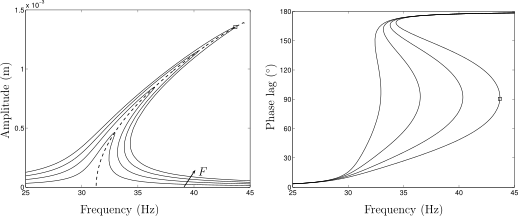
\includegraphics[width=0.7\textwidth]{nlbeam/hb/nfrc}
  \caption{Comparison between forward and backward sine sweep with HB. Sweep
    parameters: Amplitude: 3N, sweep rate: 10Hz/min. Stability is indicated for
    HB.}
  \label{fig:nlbeam_sweep}
\end{figure}

Figure \ref{fig:nlbeam_hb_components} shows the evolution of the harmonic
components along the curve. As expected from the asymmetry, there is strong
participation of the constant term, followed by the 2nd harmonic. Both due to
the squared nonlinearity.

\begin{figure}[!ht]
  \centering
  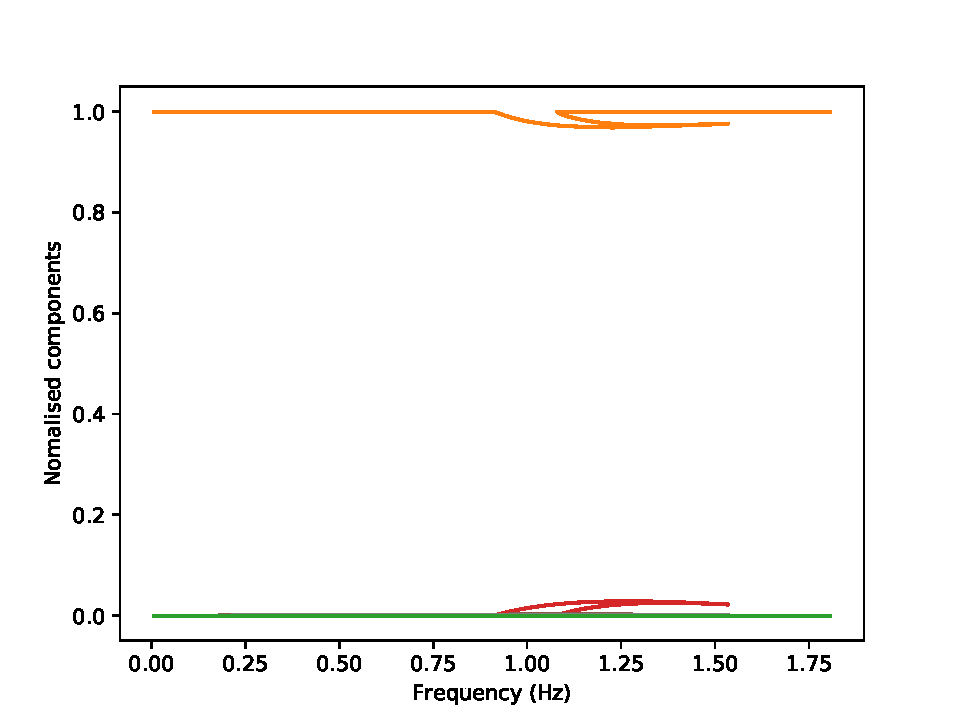
\includegraphics[width=0.7\textwidth]{nlbeam/hb/har}
  \caption{Evolution of HB components.
    \textcolor{blue}{\sampleline{}}: Constant;
    \sampleline{}: 1st;
    \textcolor{orange}{\sampleline{dotted}}: 2nd;
    \textcolor{green}{\sampleline{dash pattern=on .7em off .2em on .2em off .2em}}: 3th;
    \textcolor{red}{\sampleline{}}: 4th;
    \textcolor{purple}{\sampleline{dashed}}: 5th;
  }
  \label{fig:nlbeam_hb_components}
\end{figure}

\textbf{NNM mangler - Plot fra 1.nnm er beskrevet. 2.nnm mangler at blive beregnet.}
The NNMs of the underlying conservative system is shown in figure. The NNM
frequency increases strongly with increasing energy, which is due to the
hardening behavior of the cubic stiffness. The FEPs shows two branches emerging
from the NNM backbone. These are called tongues and are said to reveal internal
resonance. The tongue shows a 9:1 internal resonance between the first and third
NNMs.


\section{System with clearences}
\label{sec:syst-with-clear}

Ideen er at identificere clearence og parametre. Data genereres med en trilineær
model. Men da Newmark, mv. kræver at stivheden er differentiabel, bruges et
reguliseret udtryk. Det bliver forhåbent meget kortere end sidste eksempel. \textbf{Alt Mangler}.

A trilinear model for stiffness' $k_-, k, k_+$ and clearances $a_-, a_+$ is
given by, %\citet{renson2014_phd}
\begin{equation}
  \label{eq:fnl_piecewise}
  f_{nl}(x) =
  \begin{cases}
    \sign(x) \left( ka_+ + k_+(x-a_+) \right) & x \geq a_+ + \Delta_+ \\
    p_+(t(x)) & a_+ + \Delta_+ > x > a_+ - \Delta_+ \\
    kx & a_+ - \Delta_+ \geq -(a_- - \Delta_-) \\
    p_-(t(x)) & -(a_- + \Delta_-) > x > -(a_- + \Delta_-) \\
    \sign(x) \left( ka_- + k_-(x-a_-) \right) & x \leq -(a_- + \Delta_-) \\
  \end{cases}
\end{equation}
where $x$ is the relative distance between the two DOFs defining the nonlinear
connections. $2\Delta_\pm$ is the size of a regularization interval, used to
enforce continuity of the first derivative.

The Hermite polynomials $p_\pm$ are defined as
\begin{equation}
  \label{eq:fnl_herm_pol}
  p_\pm(t) = h_{00}(t)p_k + h_{10}(t)(x_{k+1}-x_k)m_k + h_{01}(t)p_{k+1} + h_{11}(t)(x_{k+1} - x_k)m_{k+1}
\end{equation}
where $p_k$ and $p_{k+1}$ are the values of the restoring force at points $x_k =
\sign(x)(a - \Delta)$ and $x_{k+1} = \sign(x)(a + \Delta)$, respectively. $m_k$
and $m_{k+1}$ are the values of the restoring force derivative at the same $x_k$
and $x_{k+1}$ points; they correspond to the stiffness coefficients k and
$k_\pm$, respectively. The local scaled abscissa and $h_{ij}$ functions are

\begin{equation}
  \label{eq:fnl_piecewise_coeff}
  \begin{aligned}
    t(x) &= \frac{x - x_k}{x_{k+1} - x_k}\\
    h_{00}(t) &=  2t^3 - 3t^2 + 1 \\
    h_{10}(t) &= t^3 - 2t^2 + t \\
    h_{01} &= -2t^3 + 3t^2 \\
    h_{11} &= t^3 - t^2 \\
  \end{aligned}
\end{equation}

Figure \ref{fig:fnl_piecewise} shows an example of a regulized nonlinear
restoring force.

\begin{figure}[!ht]
  \centering
  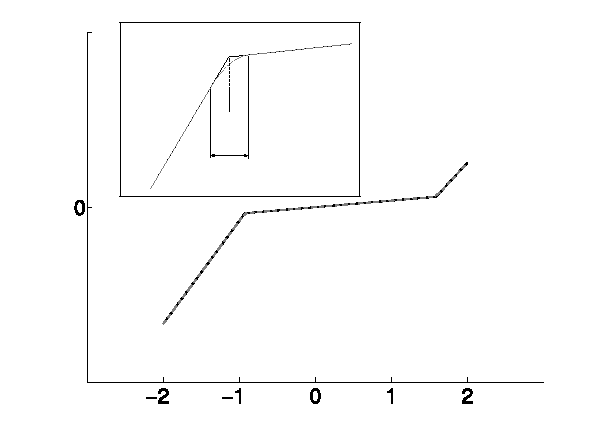
\includegraphics[width=0.7\textwidth]{appendix/piecewise_linear}
  \caption{Example of piecewise-linear restoring force. The insert image shows
    a closeup of the effect of the regularization $\Delta$.}
  \label{fig:fnl_piecewise}
\end{figure}



\FloatBarrier


%%% Local Variables:
%%% mode: latex
%%% TeX-master: "../report"
%%% End:
